\documentclass[12pt]{article}
\usepackage{a4wide}
\usepackage{sectsty}
\usepackage{graphicx}
\usepackage{enumitem,wrapfig}

\newcommand{\al}{$<$}
\newcommand{\ar}{$>$}

\parindent 0pt
\parskip 6pt

\begin{document}

\thispagestyle{empty}

\center{\huge\bf Multimodal Relational Reasoning for Visual Question Answering}
\center{\Large Computer Science Part II Project Proposal}
\center{\Large Benedict Aaron Tjandra, Trinity Hall}
\center{\Large University of Cambridge}
\center{\Large Originators: C\u{a}t\u{a}lina Cangea}

\vspace{0.3in}
\centerline{\large \emph{18 September 2019}}

\vspace{0.3in}

\flushleft{\Large \textbf{Project Supervisors:} C\u{a}t\u{a}lina Cangea}

\vspace{0.2in}

\flushleft{\Large \textbf{Director of Studies:} Prof. Simon Moore}


\vspace{0.2in}


\flushleft{\Large \textbf{Project Overseers:} Dr. Amanda Prorok, Prof. Marcelo Fiore}

\vspace{0.2in}


%\vfil%
%\eject%


\section*{Introduction and Description of the Work}

The efforts of deep learning have led to an explosive improvement in the efficiency and accuracy of mono-modal tasks. For instance, Convolutional Neural Networks (CNNs) have had great successes in object detection and segmentation \cite{fasterrcnn}, when combined with Region Proposal Networks (RPNs) and Multilayer Perceptrons (MLPs), at times surpassing human performance \cite{performance}. Recurrent Neural Networks (RNNs) have seen similar improvements when dealing with data that is sequential; for example, in audio and textual processing. These advances are necessarily \emph{mono-modal}, in that they only accept one type of input---in this case, visual or textual.

However, high-level cognitive tasks that humans perform in their day-to-day lives are \emph{multimodal}; therefore, models that aim to solve multimodal tasks require effective representations for input data sources of different types.

One example of such a task is VQA (Visual Question Answering): answering an arbitrary question about an image, which requires the comprehension of textual and visual input. 

\begin{figure}[htpb]
	\centering
	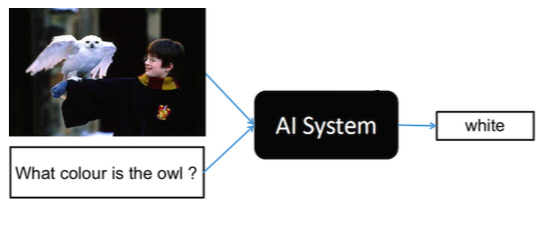
\includegraphics[scale=0.55]{vqaexample}
	\caption{
		An example of a VQA task \cite{vqaexample}.
	}
\end{figure}

This project aims to implement a network that aims to tackle VQA as described by Cadene et al. \cite{murel}. The first step is to process inputs accordingly. For the visual input, the network will use an object detection model to detect objects and their bounding boxes in the image. As for the textual input, the network will use a sentence encoder to encode the question into a vector. 

Crops of the objects detected in the image, their bounding boxes, as well as the encoded question are then fed to the MuRel cell. The latter is an atomic reasoning module that will perform bilinear fusion to combine the visual and textual inputs and construct a pairwise relational graph on which it will perform relational reasoning. The MuRel cell is unfolded for $T$ (a hyperparameter) times and then its output will be fed to the output unit. The output unit then outputs vector of probabilities over all answers that the question entails, and the answer chosen by the network is the one that is assigned the highest probability.

\begin{figure}[htpb]
	\centering
	\includegraphics[width=1.105\textwidth]{murel_net}
	\caption{
		Diagram of the MuRel network, reproduced from \cite{murel}. The network consists of an input unit, the MuRel cell, and the output unit. Here, the MuRel cell is unfolded three times before it is fed to the output unit.
	}
\end{figure}
\newpage

\section*{Resources Required}

I plan to use my own computer: a Windows laptop, equipped with 4 Intel i7 2.9GHz CPUs, 8GB RAM, and 128 GB hard disk space. The Computer Lab GPU machines will be used to conduct training, as my laptop does not have the necessary storage to install CUDA nor does it have a strong enough GPU to perform training within a tractable amount of time. If the need to use programs or command line tools that are native to Linux arises, I will be able to use a virtual machine to run Ubuntu LTS 18.04. Backups and version control of the entire project, including my dissertation, will utilise git and GitHub. 

\section*{Starting Point}

The project will rely on a working knowledge of Python, which I have obtained from the following courses:

\begin{itemize}
	\item Scientific Computing Practical Course
	\item Foundations of Data Science
\end{itemize}

The \textit{Artificial Intelligence} course contains a brief introduction to multilayer perceptrons and the backpropagation algorithm, which is a useful foundation. Additionally, I will need to familiarise myself with relevant topics and libraries, which include:

\begin{itemize}
	\item PyTorch, a library commonly used for deep learning projects
	\item Theory and practices concerning ANNs, CNNs, and RNNs
	\item Multimodal fusion methods
	\item Computer vision algorithms, e.g. object detection and classification, region proposal networks, etc.
\end{itemize}

\section*{Substance and Structure of the Project}

\subsection*{Core Objectives}
This project would mainly involve writing Python code to implement the MuRel network, as described by Cadene et al. \cite{murel}, and reproduce its results on the VQAv2 dataset \cite{vqav2}. To do this, knowledge of the PyTorch library is required, along with an understanding of CNNs, RNNs, ANNs, and knowledge of multimodal fusion methods. 

The MuRel network is comprised of modules that are connected together:

\begin{itemize}
	\item An object detection module
	\item A text encoding module
	\item The MuRel cell
	\item Multimodal fusion blocks
\end{itemize}

The object detection and text encoding modules act as feature extractors---the former will output a set of bounding boxes and crops of detected objects when given an image $I$, while the latter will output a vector that represents the semantics of a given question $Q$. These features will then be fed to a MuRel cell, which combines the features using multimodal fusion and performs relational reasoning over a number of steps $T$ to decide what answer to output. 

The current state-of-the-art object detection network, Faster-RCNN \cite{fasterrcnn}, and skipthoughts \cite{skipthoughts} will be used to detect objects in the image and encode the questions, respectively.

The project will require implementing the MuRel cell from scratch, connecting up the modules to build the MuRel network, and training the network. Training and validation will be done using the VQAv2 dataset. The size of the dataset (32 GB) is small enough to be transferred to the CL machines. However, 32 GB is quite a substantial size, and if training takes long enough to be unrealistic, it may instead be performed on a subset of the dataset. Training and validation will use GPUs, which will be provided by the Computational Biology Group at the Computer Laboratory.

\newpage

\subsection*{Evaluation}
The dataset is divided into training, validation, and test set, where each of the sets contains a collection of images, questions, and answers. Each image in the dataset is associated with several questions. The questions are open-ended, and the dataset includes 10 answers that were gathered from 10 different individuals for each question. 

For example, the 10 answers to 'What is the white streak?' are:

\begin{itemize}
	\begin{minipage}{\linewidth}
		\begin{wrapfigure}[3]{r}{0.4\textwidth}
			\item[] \begin{center}
				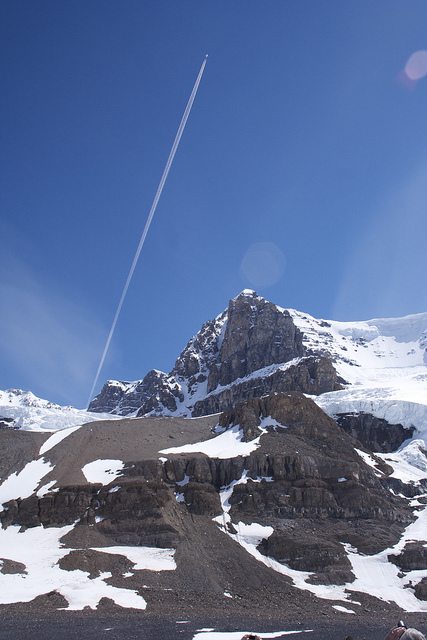
\includegraphics[width=\linewidth]{whitetrail}
			\end{center}
		\end{wrapfigure}
		\-
	\end{minipage}
	\item airplane
	\item plane trail
	\item contrail
	\item jet trail 
	\item snow
	\item contrails
	\item jet stream
	\item air trail 
	\item jet stream
	\item contrail
\end{itemize}
\vskip 10.0mm
The answers of the network to the questions in the test set will be stored in a JSON file. To evaluate the accuracy of the network, the JSON file will then be uploaded to the EvalAI website (https://evalai.cloudcv.org/), where it runs the evaluation routine to give the overall accuracy on the test set. 

The answer given by the MuRel network is compared with the answers given by the 10 individuals and the number of people that chose the answer out of 10 is then determined. The accuracy is then calculated based on this number and is maximised if at least 3 people chose that answer. To put it in equation form:

%Since each question has 10 answers, an evaluation metric that is robust to inter-human variability in how the answer is phrased is used to determine the 'correctness' or 'accuracy' of each answer:

\[Accuracy(answer) = min(\frac{\textrm{number of humans that provided that answer}}{3}, 1)\]	

To account for the variability in human judgement and to provide a more robust estimate of the network performance, accuracies given by the network for each question are evaluated over all 10 choose 9 sets of human annotators. 

To elaborate, suppose there are 10 human annotators: A, B, C, ..., J. Therefore, there are 10 possible sets of 9 human annotators --- (\{A B C D E F G H I\}, \{A B C D E F G H J\}, \{A B C D E F G I J\}, etc.). The above formula for accuracy is then applied to each set, yielding 10 accuracy values, one for each set. These 10 accuracy values are then averaged, yielding an accuracy score for a \emph{question}.

The accuracy scores for each question are then averaged to give the overall performance on the dataset.

\section*{Success Criteria}

This success of the project should be judged on the following criteria:
\begin{itemize}
	\item I have minimised the training loss function of the network on the VQAv2 dataset.
	\item The network should achieve an overall accuracy that is higher than a simple concatenation baseline, which performs concatenation of question embedding and image embedding into a single vector and feeding this vector to an MLP that does classification.
\end{itemize}

\section*{Extensions}

Should I achieve the success criteria according to or ahead of schedule, some of the following extension objectives will be attempted: 
\begin{itemize}
	\item For each object in the image, the object detection module outputs its bounding box, object crop, and its class. Currently, the MuRel network does not incorporate the object class into its computations. This extension would  incorporate the object class, either by fusion or concatenation with extracted feature vectors. The approach would likely improve performance, since the network would have more information to incorporate in the reasoning process. For example, knowing a particular crop of an image is a table will be helpful in answering questions such as 'What is on top of the table?'
	
	\item Currently, the network is given no information on the relations between objects, e.g. whether objects are on top of another. This extension will use Neural Motifs \cite{neuralmotifs} to provide the network with additional information about the relations between objects, which will hopefully improve performance as the network is given more data to work with.
	
	\item Introduce a GNN (Graph Neural Network) module for structured reasoning. Graph Neural Networks, formalised by Battaglia et al. \cite{graphnn}, provides a way to perform structured reasoning with graphs and have seen successes with problems that involve graph-like entities. For example, since we can represent chemical molecules as a graph with nodes being atoms and edges being bond length, GNNs can be used to predict whether a molecule is a medicinal drug, and hence is a potential tool for drug discovery \cite{drug}. Since the MuRel network incorporates a pairwise relational graph in its computation, this extension would introduce a GNN module to perform reasoning on the graph. This would likely improve the initial method by leveraging on the ability of GNNs to perform combinatorial generalisation.
\end{itemize}

\section*{Timetable and Milestones}

Proposed start date: 25 October 2019
\begin{enumerate}
	\item {\fontsize{12.5}{16} \textbf{Michaelmas weeks 3 to 4. 25 October 2019 - 8 November 2019}} Research the relevant theory behind ANNs, CNNs, and RNNs, how to use the PyTorch library, and read about multimodal fusion methods.
	\item {\fontsize{12.5}{16} \textbf{Michaelmas week 5. 8 November 2019 - 15 November 2019}} Obtain and write PyTorch DataLoaders for the VQAv2 dataset.
	
	Milestone: Implemented PyTorch DataLoaders for the VQAv2 dataset.
	
	\item {\fontsize{12.5}{16} \textbf{Michaelmas weeks 6 to 8. 15 November 2019 - 6 December 2019}} Prepare the object detection and text encoding module. Using the object detection module, preprocess the images in the VQAv2 dataset, and save the extracted object features to disk. Begin writing code to implement and train the MuRel network and the baseline.
	
	Milestone: Serialised processed images, image-question-answer associations, question encodings into .pth files for training. Have partially written code for the networks.
	
	\item {\fontsize{12.5}{16} \textbf{Michaelmas vacation. 6 December 2019 - 14 January 2020}} Continue writing code to implement the MuRel network. Begin training on the VQAv2 dataset. By the end of the vacation I should have implemented and trained the MuRel network and the baseline to obtain initial accuracy scores. I should also have extracted visualisations of the network reasoning, so they can be presented in the progress report presentation.
	
	Milestone: Trained the MuRel network and baseline to obtain initial accuracy scores on the dataset. Obtained several visualisations of the network reasoning.
	
	\item {\fontsize{12.5}{16} \textbf{Lent week 0. 14 January 2020 - 17 January 2020 }} Prepare progress report and progress report presentation.
	
	Milestone: Progress report and PowerPoint presentation.
	
	\item {\fontsize{12.5}{16} \textbf{Lent weeks 1 to 3. 17 January 2020 - 7 February 2020 }} Allow time to debug code and perform hyperparameter search and regularisation to improve the network's accuracy. Measure the average runtime of the network and the baseline.
	
	Milestone: Maximised the network's accuracy by doing hyperparameter search and regularisation. Measured the average runtime of the network and the baseline.
	
	\item {\fontsize{12.5}{16} \textbf{Lent weeks 4 to 6. 7 February 2020 - 28 February 2020}} Investigate extension objectives in order of difficulty, subject to the condition that the core objectives have been completed.  The first extension would be incorporating the object classes, whereas the second one would involve incorporating the scene graph. The latter is considered more difficult and involves studying Graph Neural Networks and PyTorch Geometric, a library containing GNN modules. 
	
	Milestone: Investigated extension objectives if core objectives have been completed.
	
	\item {\fontsize{12.5}{16} \textbf{Lent weeks 7 to 8. 28 February 2020 - 13 March 2020 }} Prepare the Introduction and Preparation chapters of the dissertation.
	
	Milestone: Written Introduction and Preparation chapter of the dissertation.
	
	\item {\fontsize{12.5}{16} \textbf{Easter vacation. 13 March 2020 - 21 April 2020}} Write the Implementation, Evaluation, and Conclusion chapters of the Dissertation. Send copies of the draft dissertation to Director of Studies and supervisor and amend the dissertation if necessary.
	
	Milestone: Completed the first draft of the dissertation.
	
	\item {\fontsize{12.5}{16} \textbf{Easter weeks 0 to 2. 21 April 2020 - 8 May 2020}} Make final changes to dissertation. Submit dissertation.
	
	Milestone: Dissertation submission.
\end{enumerate}

\bibliography{proposalrefs}
\bibliographystyle{ieeetr}

\end{document}
